\documentclass[a4paper]{article}

\usepackage[english]{babel}
\usepackage[utf8]{inputenc}
\usepackage{amsmath}
\usepackage{graphicx}
\usepackage[colorinlistoftodos]{todonotes}
\usepackage{fullpage}
\usepackage{graphicx}
\usepackage{caption}
\usepackage{subcaption}
\usepackage{amssymb}
\usepackage{float}
\usepackage{multicol}
\usepackage{geometry}
 \geometry{
 a4paper,
 left=20mm,
 right=20mm,
 % For multicol
 % left=15mm,
 % right=15mm, 
 top=20mm,
 bottom=20mm,
 }

\title{UCLA Computer Science Master's Comprehensive Exam: Implementation and Extension of Followship-LDA}

\author{Spencer Tung \\ Advisor: Professor Junghoo Cho}

\date{\today}

\begin{document}
\maketitle
% \begin{multicols}{2}

%%%%%%%%%%%%%%%%%%%%%%%%%%%%%%%%%%%% Abstract%%%%%%%%%%%%%%%%%%%%%%%%%%%%%%%%%%
\begin{abstract}
asdf
\end{abstract}

%%%%%%%%%%%%%%%%%%%%%%%%%%%%%%%%%%%% Section 1: Project Idea%%%%%%%%%%%%%%%%%%%%%%%%%%%%%%%%%%
\section{Introduction}
Semantic analysis, the art of getting computers and programs to understand the meaning behind text, has been a long standing problem in computer science. There can be many practical applications of semantic analysis, such as identifying the topics that comprise a given document. This, in turn, could be used to determine what sort of topics the reader of this document is potentially be interested in. In today's advertisement-driven and consumer-focused world, being able to automatically obtain this information, independent of the source, is invaluable.

These days, there is a large amount of traffic centered around social media, which many advertisers leverage to market their products. Twitter is one such social media site, focused on microblogs of 140 characters or less. Every time a Twitter user submits a post, known as a \textit{tweet}, the tweet is blasted out to all of the other users that have chosen to \textit{follow} this specific user. The information flow is therefore generated by the \textit{followee} and received by the \textit{follower}. On a microblog site such as Twitter, it can be difficult for marketers to determine where their ads will have the most weight, as there are literally millions of tweets coming from millions of users every day \cite{TODO}. Knowing who key influencers are on Twitter goes a long way for advertisers, who can be more selective about how they reach out to their audience.

However, there are some advertisers who, instead of taking the time to do their own research and fine tune their efforts, will resort to more widespread methods to attract followers. This will often take the form of a computer scipt that blasts their advertisements to anyone who follows them. Known as \textit{Twitterbots}, or spambots to most, these drones are often viewed as being annoyances to legitimate users who may not care for the bot tweets. It is therefore advantageous to be able to automatically identify whether a user is legitimate or a bot and take appropriate measures accordingly.

This paper will focus on an extension of \textit{Latent Dirichlet Analysis} (LDA). LDA is a probabilistic topic model, and can be applied to a set of documents (known as a \textit{corpus}) to extract topic information for each document and every word in a given corpus. The extension of this model, known as \textit{Followship-LDA} (FLDA), leverages Twitter follower-followee network information to identify either important and influential entities on Twitter, or spambots that most people won't pay attention to and should remove from their followee list. The details of both models will be discussed in Section \ref{sec:prevwork}.

The paper will be organized as follows. Section \ref{sec:prevwork} will discuss any previous work that came before this paper. Most importantly, it details the FLDA method critical to algorithm's success. Section \ref{sec:approach} will discuss the system architecture and design. Section \ref{sec:results} will detail the results of running the FLDA model on the Twitter data subset. Finally, Section \ref{sec:conc} will discuss the conclusions.

% \subsection{Motivation}
% I chose this project to further my understanding of semantic analysis, as well as challenge myself by implementing an algorithm that could efficiently deal with big data.


%%%%%%%%%%%%%%%%%%%%%%%% Section 2: Methodology and Previous Work%%%%%%%%%%%%%%%%%%%%%%%%%%%
\section{Background and Previous Work}
\label{sec:prevwork}
\subsection{Overview}
To understand how FLDA works, it is necessary to first gain an understanding of how LDA works. As mentioned previously, LDA is a type of probabilistic topic model, which is one approach for semantic analysis. These are models that operate under the following assumptions: that a document is a mixture of different topics, and each topic is a distribution of words. As these are \textit{generative models} for documents, it demonstrates a probabilistic procedure that can be used to generate various documents. Table \ref{tab:ldatopics} shows two example topics, ranked by top 4 words that have a high probability of belonging to that topic. Note that although neither topic is labeled, it is clear to see that Topic 1 most likely has to do with fictional works, whereas Topic 2 revolves around plants and nature. To generate documents from these topics, one simply assigns a probability to each topic and selects words based on the probability distribution of the words in the topics \cite{lda}. In this example, by assigning an equal probability to both topics in this table, one could generate a document that talked about the fictional story of a tree who wanted a bee to come along and pollinate his flowers.

\begin{table}[h]
  \centering % used for centering table
  \begin{tabular}{ |l|l|l|l|l| }
    \cline{0-1}
    \cline{4-5}
    \multicolumn{2}{|l|}{\textbf{Topic 1}} & & \multicolumn{2}{|l|}{\textbf{Topic 2}} \\
    \cline{0-1}
    \cline{4-5}
    word & prob & & word & prob \\
    \cline{0-1}
    \cline{4-5}
    BOOK & 0.06 & & TREE & 0.04 \\
    NOVEL & 0.04 & & FLOWERS & 0.03 \\
    STORY & 0.03 & & POLLEN & 0.03 \\
    HARDCOVER & 0.01 & & FRUIT & 0.02 \\
    \cline{0-1}
    \cline{4-5}
  \end{tabular}
  \caption{Two inferred topics as a result of running LDA on a given corpus. These topic probabilities can also in turn be used to generate documents by selecting words from each topic.}
  \label{tab:ldatopics}
\end{table}

Using statistical techniques, it is possible to invert this process and infer the set of topics that were used to generate the documents in question. That is, given a set of documents, one could return a list of topics, each with their own probability distribution of likely words. This is the process known as LDA.

\subsection{LDA}
To start, we first define some variables and equations. $P(z)$ is the probability distribution of topics $z$ over a given document - an example of this would be the equal document we generated previously. There, both topics 1 and 2 had a $50\%$ probability of showing up in the document. $P(w | z)$ is the probability of word $w$ being chosen, given topic $z$. This would be represented by the probabilities listed in Table \ref{tab:ldatopics}. More common or otherwise prominent words for a topic $z$ are given higher weights that the less used ones. A document can therefore be generated, word by word, by first selecting a topic from the distribution of topics, and then sampling a word $w_i$ from the topic-word distribution $P(w | z)$. We represent these two actions with $P(z_i = j)$, which is the probability that for the $i$th word token in a given document, the $j$th topic was selected, and $P(w_i | z_i = j)$, which is the probability of word $w_i$ in topic $j$'s word distribution.

We can simplify the notation using $\phi^{(j)}$ to represent this multinomial distribution of the words for topic $j$, and $\theta^{(d)}$ to represent the multinomial distribution of topics for document $d$. In essence, $\phi$ denotes which words are important for a given topic, and $\theta$ will list out the important topics for a given document. Finally, given that we are inferring these document-topic and topic-word distributions with no prior information about the corpus (ie. the set of documents), we must select a total number of topics $T$ for our inference. The total number of documents in the corpus is $D$, where each document $d$ consists of $N_d$ words, and the total number of words is $N$, where $N = \sum\limits^D{N_d}$ \cite{lda}. Table \ref{tab:ldavars} lists out the aforementioned variables for easy reference.
\begin{table}[h]
  \centering % used for centering table
  \begin{tabular}{ |l|l| }
    \hline
    Notation & Description \\
    \hline
    \hline
    $P(z)$ & Distribution of topics $z$ over a given document \\
    $P(w | z)$ & Distribution of words $w$ over a given topic $z$ \\
    $P(z_i = j)$ & Probability that topic $j$ was sampled for the $i$th word in a given document \\
    $P(w_i | z_i = j)$ & Probability of word $w_i$ for topic $j$ \\
    $\phi^{(j)}$ & Simplified representation of $P(w | z = j)$, for topic $j$ \\
    $\theta^{(d)}$ & Simplified representation of $P(z)$, for document $d$ \\
    $w_i$ & $i$th word in a document \\
    $T$ & Number of topics, manually chosen \\
    $D$ & Number of documents in the corpus \\
    $N_d$ & Number of words in document $d$ \\
    $N$ & Number of words in the corpus \\
    \hline
  \end{tabular}
  \caption{Quick reference for notation and variables used in LDA}
  \label{tab:ldavars}
\end{table}

Given the document-topic and topic-word probability distributions, we can subsequently define the probability distribution of each word in a document with $P(w_i)$, in Equation \ref{eq:lda_probdist}.

\begin{equation}\label{eq:lda_probdist}
  P(w_i) = \sum\limits_{j=1}^T P(w_i | z_i = j) P(z_i = j) = (\phi^{(j)}_i) (\theta^{(d)}_i)
\end{equation}

As the number of topics is manually specified by the user, this operation's space and time complexity is constrained by $T$. If we extend the visualization from Table \ref{tab:ldatopics} (simplified as $\phi$), we can imagine $\phi$ as a 2D matrix, with each word token index represented by the row indices $i$, the topic indices represented by the column indices $j$. The entries of this matrix are then the probabilities of word $i$ being assigned to a topic $j$. We use a similar definition to define $\theta$, where the entries of this 2D matrix are the probabilities of topic $i$ being assigned to document $j$. Figure \ref{fig:topicmodel} gives a visual representation of Equation \ref{eq:lda_probdist}. It is clear to see from Figure \ref{fig:topicmodel} that it is important to choose an appropriate value for $T$ in order to have meaningful results for $\theta$ and $\phi$ \cite{lda}.

\begin{figure}[h]
  \centering
    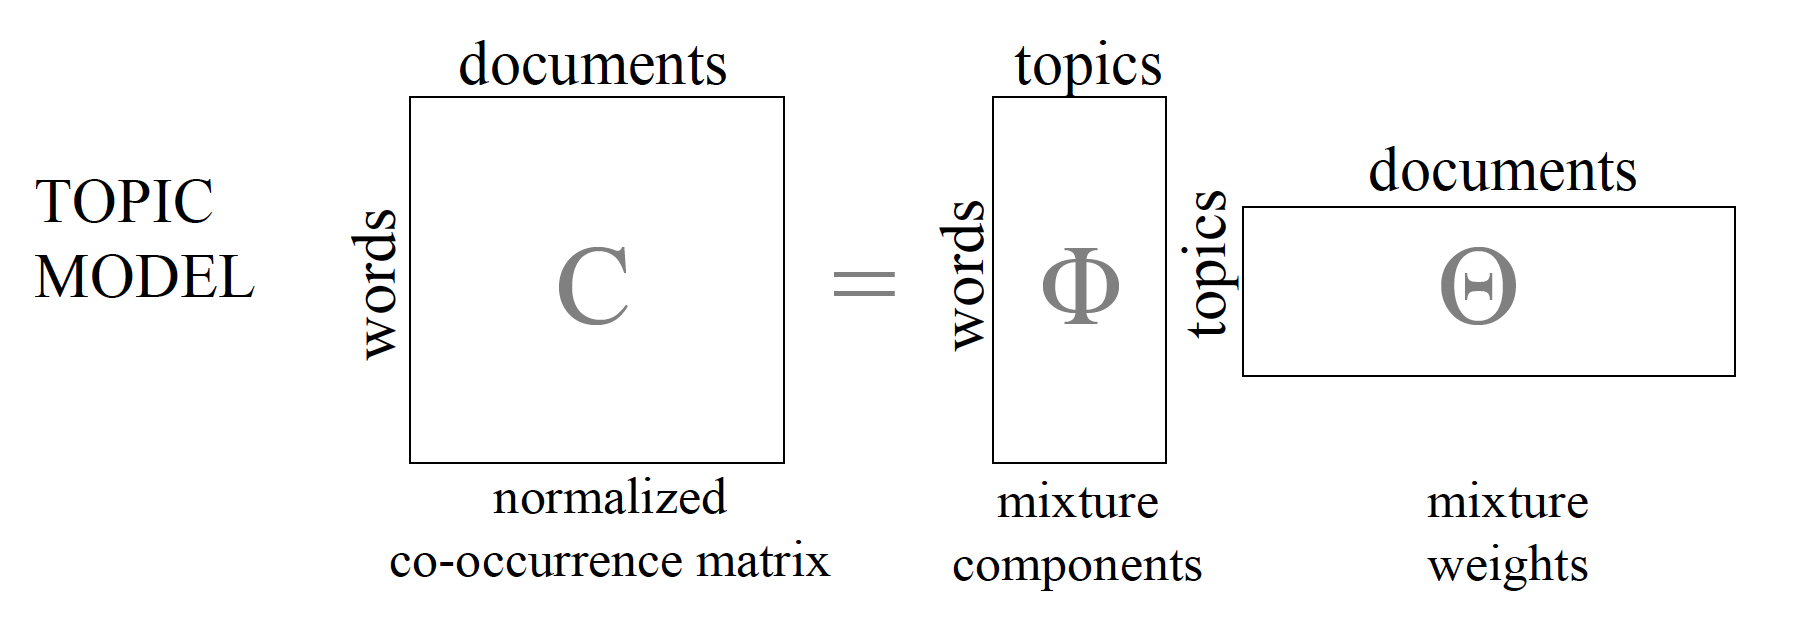
\includegraphics[width=0.7\textwidth]{topicmodel}
  \caption {Visual representation of the probabilistic topic model}
  \label{fig:topicmodel}
\end{figure}

LDA distinguishes itself from other probabilistic topic model by including a \textit{Dirichlet prior} on the $\theta$ parameter. The use of a prior allows for the algorithm to make a general assumption about how its weights are generated, based on the total number of topics chosen \cite{hoffman}. As the Dirichlet distribution is a conjugate prior for the multinomial distribution, this means that the posterior distribution will also be a Dirichlet. In addition, it is relatively simple to sample from the Dirichlet distribution. While a detailed explanation of conjugate priors is outside of the scope of this paper, we will turn our focus instead to the portions that will allow us to implement LDA \cite{lda}. It is sufficient to know that the Dirichlet distribution is used to model the multinomial distribution of $\theta$, and the parameters of the Dirichlet distribution are known as \textit{hyperparameters}, distinguishing them from the parameters $\theta$ and $\phi$ of the underlying distribution. In our situation, each hyperparameter $\alpha_j$ from $\alpha_1, ..., \alpha_T$ represents the initial, prior count for the number of times topic $j$ was sampled in a document. A similar hyperparameter $\beta$ is assigned to model $\phi$ as well, representing the prior count for the number of times a word was sampled from a topic. It is important to remember that this occurs before we have even begun the actual sampling process.

\subsection{Gibbs Sampling}
As mentioned in the previous section, one of the reasons a Dirichlet prior is included is because it is simple to sample from a Dirichlet distribution. While it is possible to directly estimate the parameters $\theta$ and $\phi$, this has a tendency of converging on local maxima, leading to results that may differ wildly from run to run \cite{hoffman}. Instead, LDA takes all of the observed words in the corpus, $w$, and uses them to create the posterior distribution of $z$, which we define as the topic assigned to each word. For each $w_i$, a topic (represented by an integer value from $1, ..., T$) $z_i$ is assigned to it. When it comes to dealing with a corpus that includes millions of words, Gibbs sampling is an efficient and simple method of achieving our goals in a reasonable time frame \cite{lda}.

Gibbs sampling utilizes \textit{Markov Chain Monte Carlo} (MCMC), which builds its next response based on the results of the previous iteration. This process continues until the requisite number of iterations has been fulfilled (as manually specified by the user), or when the results have converged and do not vary drastically from iteration to iteration. As this procedure does not directly estimate the values of $\theta$ and $\phi$, they can be estimated once $z$ has converged.

Equation \ref{eq:lda_gibbssamp} shows one such example of a Gibbs sampling equation, given by Griffiths and Steyvers \cite{griff}.

\begin{equation}\label{eq:lda_gibbssamp}
  P(z_i = j | z_{-i}, w_i, d_i, \cdot) \propto
    (\frac{C_{w_ij}^{WT} + \beta}
    {\sum\limits^W_{w = 1} C_{wj}^{WT} + W\beta})
    (\frac{C_{d_ij}^{DT} + \alpha}
    {\sum\limits^T_{t = 1} C_{d_ij}^{DT} + T\alpha})
\end{equation}

The terms $C_{wj}^{WT}$ and $C_{dj}^{DT}$ denote the two count matrices used for inferring the parameters. They represent the number of times word $w$ is assigned to topic $j$, and the number of times topic $j$ was assigned to a word in document $d$, respectively. Note that both matrices exclude the current instance $i$ - this is to remove the influence of the current instance on the total distribution when sampling for a new topic for that specific instance. All of the other terms in Equation \ref{eq:lda_gibbssamp} have previously been introduced - the ``$\cdot$'' notation represents all other known variables, which are unchanged \cite{lda}.

As one can see, the premise of the sampling equation works by checking both how likely a given word is for a topic, as well as how dominant a given topic is in a document. The left side of the equation checks the probability of the word in the topic against all of the other words in the topic, while the right side of the equation checks the given topic against the other topics in the document. While we intialize these count matrices randomly, given enough iterations, words that show up consistently in the same document will begin to converge in topic groups, which will influence the topic distribution of that document, as well as the word distribution of the topics too. This will decrease the irrelevant topic assignments while increasing the number of relevant groupings over time \cite{lda}.

As such, we can also estimate our $\phi$ and $\theta$ variables by splitting the sampling equation in those two respective parts. Recall that our Gibbs sampling equation, Equation \ref{eq:lda_gibbssamp}, only provides an estimate for $z$, the probability that topic $j$ is sampled for a given word $w_i$. What is usually of greater interest are the topic probability distributions, $\phi$ and $\theta$. Equation \ref{eq:lda_phi} utilizes the topic-word count matrix $C_{wj}^{WT}$ to obtain the topic-word probability distribution, and Equation \ref{eq:lda_theta} utilizes the document-topic count matrix $C_{dj}^{DT}$ to obtain the document-topic probability distribution \cite{lda}.

\begin{equation}\label{eq:lda_phi}
  \phi'^{(j)}_i = (\frac{C_{w_ij}^{WT} + \beta}
  {\sum\limits^W_{w = 1} C_{wj}^{WT} + W\beta})
\end{equation}

\begin{equation}\label{eq:lda_theta}
  \theta'^{(d)}_j = (\frac{C_{d_ij}^{DT} + \alpha}
  {\sum\limits^T_{t = 1} C_{d_ij}^{DT} + T\alpha})
\end{equation}

Once these distributions have been estimated from our sampled $z$, we are able to provide a list of topics, along with the words that have the highest likelihoods of being in each topic, which should all have some relation to one another. This is the basic essence of the semantic analysis method LDA.

\subsection{FLDA}
FLDA extends this LDA model by incorporating an analysis on the microblog network as well, identifying persons of interest within the aforementioned topics. This can either be people with a lot of influence over certain topics, as was the case in Bi et al \cite{flda}, or identifying potential spammers, which is the direction this paper will be taking. Though there have been other attempts to model topic influencers on a microblog network, FLDA differs from its predecessors in that it takes into account the notion that some users may follow other users for their popularity alone, independent of content. This important distinction helps decrease the influence of other users who are prominent in certain topics, who follow famous users not because they are interested in the topics that they blog about, but simply because they are celebrities \cite{flda}.

To that end, we identify new notation for the extra variables we need to keep track of for FLDA. We now have an $x$ variable that tracks the identity of the topic of someone the given user is following, as well as a $y$ the stores the binary indicator of whether the given user is following someone for their content or not. In addition to the original $\theta$ and $\phi$ topic distributions, we now have $\sigma$, which tracks the topic probability distribution of each follower for the given topic, $\mu$, which tracks the indicator distribution over each user, and finally $\pi$, which stores the probability of a given user being followed for non-content reasons (ie. being famous) \cite{flda}. As before, the new notation introduced here is listed in Table \ref{tab:fldavars} for easy reference.

\begin{table}[h]
  \centering % used for centering table
  \begin{tabular}{ |l|l| }
    \hline
    Notation & Description \\
    \hline
    \hline
    $x$ & Identity of the topic given the follower \\
    $y$ & Binary value indicating whether the follower relationship is based on content or not \\
    $\sigma$ & Probability that a follower is assigned a given topic for this specific user \\
    $\mu$ & Binary distribution (Bernoulli) over the content indicators \\
    $\pi$ & Global popularity probability distribution over the links of each user \\
    \hline
  \end{tabular}
  \caption{Quick reference for notation and variables used in FLDA}
  \label{tab:fldavars}
\end{table}

The Gibbs sampling equations for FLDA have also been tweaked from the original LDA, as they need to not only incorporate the semantic analysis of the topics in the tweets, but also the topic analysis of the followship network as well. The notation used to represent our matrices in these equations are as follows: $c_{z, m, w}$ is a 3D matrix that represents the number of times word $w$ was assigned to topic $z$ for user $m$, and $d_{x, m, e, y}$ is a 4D matrix that represents the number of times link $e$ was assigned to topic $x$ by user $m$, given the content indicator $y$ (remember that if $y$ is $0$, then user $m$ is following link $e$ for non-content reasons, and if $y$ is $1$, then the link is followed for content reasons) \cite{flda}.
\begin{equation}\label{eq:flda_sem}
  \begin{gathered}
    p(z_{m, n} | z_{-(m, n)}, x, w, e, y, \alpha, \beta, \gamma, \epsilon, \rho) \propto \\
      \frac{(c_{z_{m, n}, m, *}^{-(m, n)} + d_{z_{m, n}, m, *, *} + \alpha_{z_{m, n}})
      (c_{z_{m, n}, *, w_{m, n}}^{-(m, n)} + \beta_{w_{m, n}})}
      {c_{z_{m, n}, *, *}^{-(m, n)} + \sum^W_{i = 1}\beta_i}
  \end{gathered}
\end{equation}

\begin{equation}\label{eq:flda_net_0}
  \begin{gathered}
    p(x_{m, l}, y_{m, l} = 0 | y_{-(m, l)}, x_{-(m, l)}, w, z, e, \alpha, \beta, \gamma, \epsilon, \rho) \propto \\
      (c_{x_{m, l}, m, *} + d_{x_{m, l}, m, *, *}^{-(m, l)} + \alpha_{x_{m, l}})(d_{*, m, *, 0}^{-(m, l)} + \rho_0) \times
      \frac{d_{*, *, e_{m, l}, 0}^{-(m, l)} + \epsilon_{e_{m, l}}}
      {d_{*, *, *, 0}^{-(m, l)} + \sum^M_{i = 1}\epsilon_i}
  \end{gathered}
\end{equation}

\begin{equation}\label{eq:flda_net_1}
  \begin{gathered}
    p(x_{m, l}, y_{m, l} = 1 | y_{-(m, l)}, x_{-(m, l)}, w, z, e, \alpha, \beta, \gamma, \epsilon, \rho) \propto \\
      (c_{x_{m, l}, m, *} + d_{x_{m, l}, m, *, *}^{-(m, l)} + \alpha_{x_{m, l}})(d_{*, m, *, 1}^{-(m, l)} + \rho_1) \times
      \frac{d_{x_{m, l}, *, e_{m, l}, 1}^{-(m, l)} + \gamma_{e_{m, l}}}
      {d_{x_{m, l}, *, *, 1}^{-(m, l)} + \sum^M_{i = 1}\gamma_i}
  \end{gathered}
\end{equation}

Here, Equation \ref{eq:flda_sem} creates a distribution for the topic assignment of the given word $z_{m, n}$, where $z$ is the topic-word identity matrix mentioned before, and the indices indicate that this is the assignment for the $n$th word of the $m$th user. Equation \ref{eq:flda_net_0} creates the distribution $x$ for the $l$th followship link of the $m$th user, given that the user is following the link for non-content reasons (ie. $y = 0$). Equation \ref{eq:flda_net_1} thereby creates the $x$ distribution for the same indices, but instead given that the user is following the link for content-dependent reasons (ie. $y = 1$). All of these distributions are then uniformly sampled to produce the count matrices used to estimate the probability distributions, which are shown in Equations \ref{eq:flda_theta} to \ref{eq:flda_pi} for reference purposes. These are the equations used to estimate the distribution parameters, from which we can obtain the words and people of interest under each topic subcategory.

\begin{equation}\label{eq:flda_theta}
  \theta_{x | m} = \frac{c_{x, m, *} + d_{x, m, *, *} + \alpha_x}{c_{*, m, *} + d_{*, m, *, *} + \sum_{i = 1}^K\alpha_i}
\end{equation}
\begin{equation}\label{eq:flda_phi}
  \phi_{w | z} = \frac{c_{z, *, w} + \beta_w}{c_{z, *, *} + d_{*, m, *, *} + \sum_{i = 1}^W\beta_i}
\end{equation}
\begin{equation}\label{eq:flda_mu}
  \mu_{y | m} = \frac{d_{*, m, *, y} + \rho_y}{d_{*, m, *, *} + \rho_0 + \rho_1}
\end{equation}
\begin{equation}\label{eq:flda_sigma}
  \sigma_{e | x} = \frac{d_{x, *, e, 1} + \gamma_e}{d_{x, *, *, 1} + \sum_{i = 1}^M\gamma_i}
\end{equation}
\begin{equation}\label{eq:flda_pi}
  \pi_{e} = \frac{d_{*, *, e, 0} + \epsilon_e}{d_{*, *, *, 0} + \sum_{i = 1}^M\epsilon_i}
\end{equation}

The next section will discuss the implementation details of my project.

%%%%%%%%%%%%%%%%%%%%%%%% Section 3: System Design and Approaches%%%%%%%%%%%%%%%%%%%%%%%%%%%%%
\section{System Design and Approaches}
\label{sec:approach}
\subsection{System Architecture Overview}
Given that LDA is already a well known model, there are many existing open source implementations readily available. To narrow the scope of my project, I chose to use the gibbsLDA \verb!C++! implementation \cite{gibbs_lda}, understand the code, and use that as a baseline from which to extend and model the followship network analysis from. This way, I would be able to focus only on implementing a working version of the FLDA described in Bi's paper \cite{flda}.

The gibbsLDA implementation was tested on the Twitter dataset to verify that the LDA algorithm works on a microblog network (more details in section \ref{sec:data} and \ref{sec:challenges}). From there, new functions were added, modeled after the existing LDA counterparts. A new mode was added to the software package, so that the option to run either LDA or FLDA were present. The only new options that were included in the FLDA mode were an option to print out the top $n$th people of interest in a particular topic (be they highly influential people or spammers, depending on the direction of followers), and a follower file that listed out either the people who the given user is following, or people that are following the given user.

The critical part of the implementation lay in the new sampling equations, as they determined the distributions from which each of the variables would sample. As Equation \ref{eq:flda_sem} was a direct counterpart to Equation \ref{eq:lda_gibbssamp} in regular LDA, the implementation details of Equation \ref{eq:flda_sem} were relatively straightforward. Both equations concerned themselves with semantic content and extracting topic information from a corpus, so this was no surprise. Equations \ref{eq:flda_net_0} and \ref{eq:flda_net_1}, however, ventured into new territory, as they modeled two different variables together. It was therefore necessary to create a single distribution from the two sampling equations, and extract both the content indicator and topic variables from the single distribution. This was accomplished by merging the two distributions generated from the two equations together and obtaining both sampled results from this merged distribution (the details of which are discussed in \ref{sec:samp_eqns}). Depending on what the current content indicator value was, the appropriate count matrices were decremented before the start of each distribution generation, and re-incremented depending on what the newly sampled content indicator value was.

As the original open source implementation only concerned itself with 2D matrices, it became necessary to find a reasonable way to represent the 3D and 4D matrices shown in the FLDA paper. To accomplish this, multiple 1D and 2D arrays were used to represent the 3D and 4D matrices $c_{z, m, w}$ and $d_{x, m, e, y}$ respectively. These arrays aggregate the entries in the unrepresented dimension(s), thereby reducing the dimensions of a very large matrix. This greatly increases the speed at which the algorithm can run, though at the obvious cost of requiring more space to store redundant information.

All prior values were set to 0.1, except for $\alpha$, which was set to $50.0 / K$, and $\rho$, which was set to $1$. The former is a standard value to set $\alpha$ to in LDA \cite{lda}, and the latter is the value that was used in the original FLDA runthrough \cite{flda}. 

Other pre-processing details to note were remembering to put the total number of lines in the corpus and followers files at the top of file. This tells the \verb!C++! code how much memory to allocate for the main arrays that store all of the corpus and follower information that the FLDA needs.

\subsection{Data Sources}\label{sec:data}
Twitter was chosen as the microblog in question. While the original Twitter data used is 8 GB large, a much smaller subset weighing in at about 100MB was used to test the algorithm.

Describe how LDA and FLDA work on the dataset

\subsection{Challenges}\label{sec:challenges}

\subsubsection{Data Cleaning}
I obtained the two Twitter datasets from Zijun. 
I worked with another student on cleaning the tweets from each individual user. I removed usernames 

TODO: remove non-ASCII characters (hopefully most remaining tweets will be in English, or at least Western languages)
remove words that appear in less than X tweets

Creating Amazon EC2 instance (list out specs)

Can only test followee network on full dataset because sub-datasets have low overlap

ssh broken pipe problems

% Modifying the sampling distribution for Eqn2 and 3
\subsubsection{Sampling Equations}\label{sec:samp_eqns}
As the Gibbs LDA source code already included an example of a sampling equation, it was simple to modify the code to account for the extra variables in Equation \ref{eq:flda_sem} \cite{gibbs_lda}. Equations \ref{eq:flda_net_0} and \ref{eq:flda_net_1} required a little more ingenuity. With a little help from Zijun to interpret the sampling equations in the paper, I created both distributions, then created a cumulative sum of both distribution probabilities for uniform sampling. The size of this cumulative distribution would therefore be twice the size of the total number of topics, $K$. Therefore, if the topic index sampled exceeded $K$, we would subtract $K$ from the value to normalize it (as the topic indices between the two equations refer to the same topics) \cite{flda}.

%%%%%%%%%%%%%%%%%%%%%%%%%%%%%%%%% Section 4: Set Up and Results%%%%%%%%%%%%%%%%%%%%%%%%%%%%%%%
\section{Results}
\label{sec:results}
\subsection{Preliminary Results}
As I was extending an existing software package, I needed to ensure that the original program would reliably run LDA on a modified dataset.


%%%%%%%%%%%%%%%%%%%%%%%%%%%%%% Section 5: Evaluation and Discussion%%%%%%%%%%%%%%%%%%%%%%%%%%%
\section{Conclusions and Future Work}
\label{sec:conc}

As described by Bi et al. in \cite{flda}, it is possible to implement FLDA in such a way that allows for parallelization. The implementation done by their group leveraged Spark, a framework that 

As Spark comes with built in Java support, it would have required a different approach to 

%%%%%%%%%%%%%%%%%%%%%%%%%%%%%%%%%%%% Section 6: Teamwork%%%%%%%%%%%%%%%%%%%%%%%%%%%%%%%%%%%%%%
\section{Miscellaneous}
\label{sec:misc}
\subsection{Programming Languages}
Two programming languages were used in this project:
\begin{enumerate}
\item \textbf{Python}: This was used to process the Twitter dataset. The corpus information from the tweets was organized, as well as the friend network information. Extraneous words and words from other languages were also filtered out, to the best of my ability.
\item \textbf{C++}: This was used to do all of the algorithmic work for FLDA, such as initialization, sampling, and estimation of the final variables. The Gibbs LDA source code in C++ was used as a starting point for the FLDA functions.
\end{enumerate}

% \end{multicols}

\begin{thebibliography}{9}
% APA Style
\bibitem{flda}
Bi, B., Tian, Y., Sismanis, Y., Balmin, A., \& Cho, J. (2014, February). Scalable topic-specific influence analysis on microblogs. In \textit{Proceedings of the 7th ACM international conference on Web search and data mining} (pp. 513-522). ACM.

\bibitem{griff}
Griffiths, T. L., \& Steyvers, M. (2004). Finding scientific topics. \textit{Proceedings of the National Academy of Science, 101}, 5228-5235.

\bibitem{hoffman}
Hofmann, T. (1999, August). Probabilistic latent semantic indexing. In \textit{Proceedings of the 22nd annual international ACM SIGIR conference on Research and development in information retrieval} (pp. 50-57). ACM.

\bibitem{lda}
Steyvers, M., \& Griffiths, T. (2007). Probabilistic topic models. \textit{Handbook of latent semantic analysis}, 427(7), 424-440.

\bibitem{gibbs_lda}
Xuan-Hieu Phan and Cam-Tu Nguyen. GibbsLDA++: A C/C++ implementation of latent Dirichlet allocation (LDA), 2007

\bibitem{TODO}
YOU NEED TO CITE ALL OF THESE SOURCES

\end{thebibliography}

\end{document}